\documentclass[11pt,a4paper]{article}
\usepackage[text={6.5in,10in},centering,a4paper]{geometry}
\usepackage{amssymb,amsmath} % Equations
\usepackage{tabularx} % Tables
\usepackage{graphicx,color} % Graphics, Figures
\usepackage[tight,footnotesize]{subfigure}
\usepackage{pgfgantt}           % for gantt chart
\usepackage{hyperref}
%\usepackage[no-math]{fontspec}

\graphicspath{{figures/}} % create a director 'figures' in your local dir and all pics are kept here


\title{\bf Senior Project Report 2102499 Year 20XX  \\[2ex]
Solar irradiance forecasting for Chulalongkorn University location using time series models
}
\author{ \bf Justin Bieber ID XXXX  \\[1ex]
\bf Advisor: Assist. Prof. Jitkomut Songsiri \\[1ex]
\bf Department of Electrical Engineering, Faculty of Engineering \\[1ex]
\bf Chulalongkorn University
}
\date{}

\renewcommand\familydefault{\sfdefault} % set to San Serif series

\begin{document}
\maketitle

\begin{abstract}
This template is for preparing the senior project report in English. The guideline of writing the contents can be read from the Thai template. 
\end{abstract}

\paragraph{\textbf Keywords:} solar forecasting, ARIMA models (up to five) \\

% Note: the abstract should be fit in the cover

\newpage
\tableofcontents




\newpage
\section{Introduction}

\section{Project Overview}
\subsection{Objectives}
\subsection{Scope of Work}
\subsection{Expected Outcomes}

\section{Methodology}
\label{sec:principle}

\section{Results}

\section{Conclusions}

\section{Acknowledgement}
(optional)



\section{List of LaTeX usage}

\subsection{Tables}
\begin{table}[ht]
\centering
\caption{Example} 
\vspace{3mm}
\begin{tabular}{|l|c|c|r|} \hline
Item & Font & Font Type & Font Size \\ \hline
Title &Garamond &Bold &20  \\
Author names & Garamond & Bold & 12 \\ 
Author affiliation/email & Garamond & Regular & 11 \\
Abstract/Keywords & Garamond & Regular & 11 \\
Level 1 headings & Garamond & Bold & 12 \\
Level 2 headings &Garamond & Bold & 11 \\
Level 3 headings & Garamond & Regular & 11 \\
Figure/table captions & Garamond & Regular & 11 \\
Main text/References & Garamond & Regular & 11 \\ \hline
\end{tabular}
\end{table}

\subsection{Figures}

\begin{figure}[ht]
	\begin{center}
		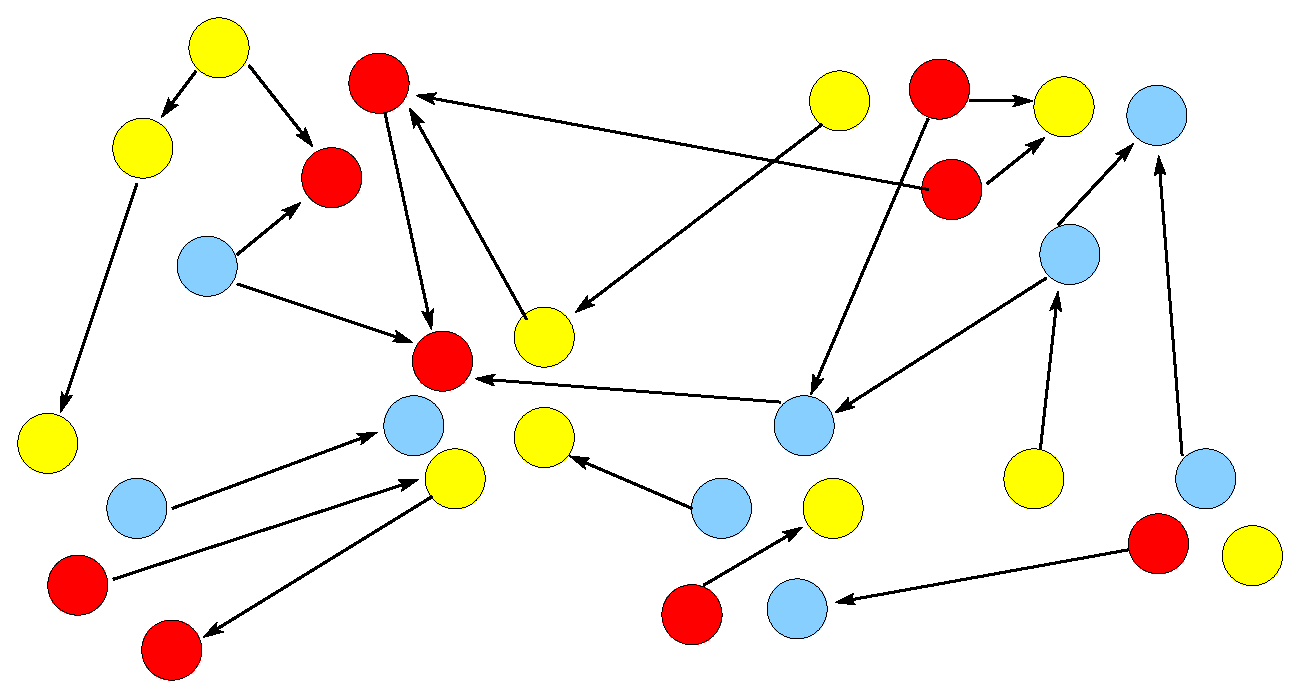
\includegraphics[width=0.7\linewidth]{gm.eps}
		\caption{แบบจำลองเชิงกราฟ}
	\end{center}
\end{figure}

\begin{figure}[h!]
	\begin{center}
		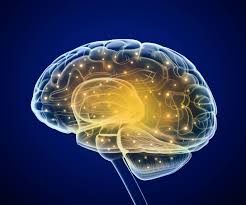
\includegraphics[width=0.5\linewidth]{brain.jpg}
		\caption{สภาพการเชื่อมโยงของสมอง (Source: Shutterstock.com Image by: Alex Mit)}
	\end{center}
\end{figure}

\begin{figure}
\centering
\subfigure[first caption]{ 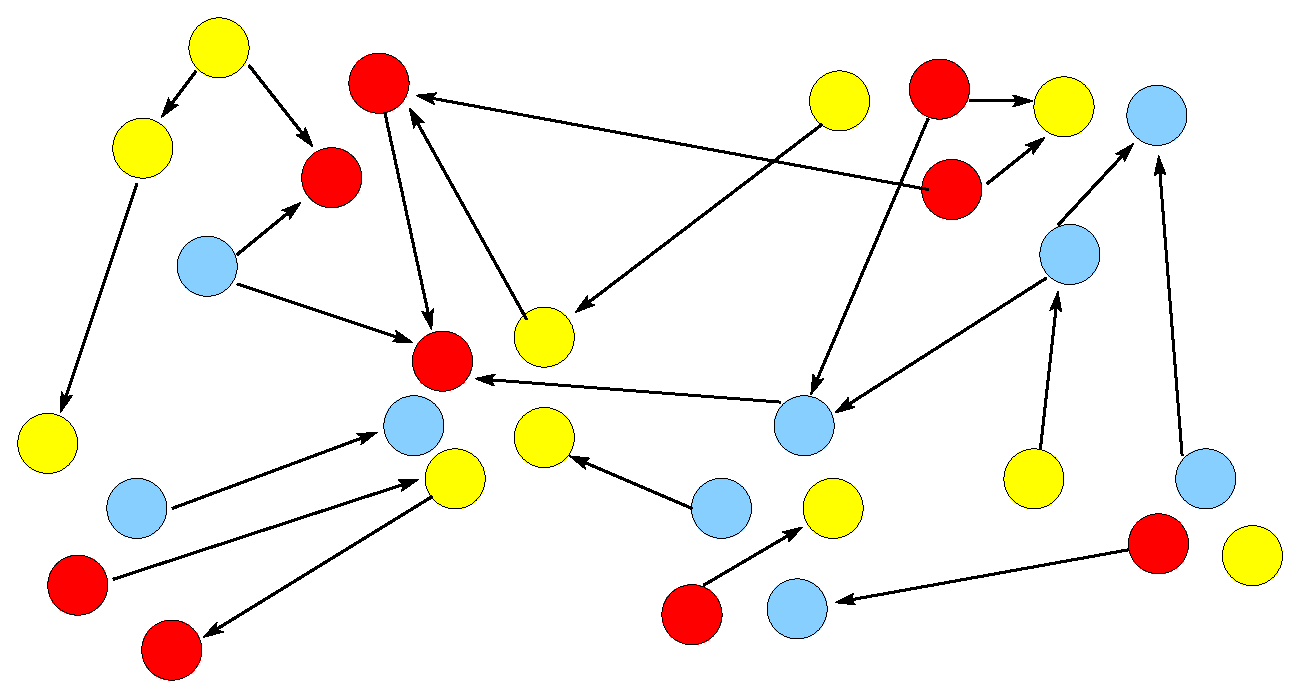
\includegraphics[width=0.45\linewidth]{gm.eps}  } 
\subfigure[second caption]{ 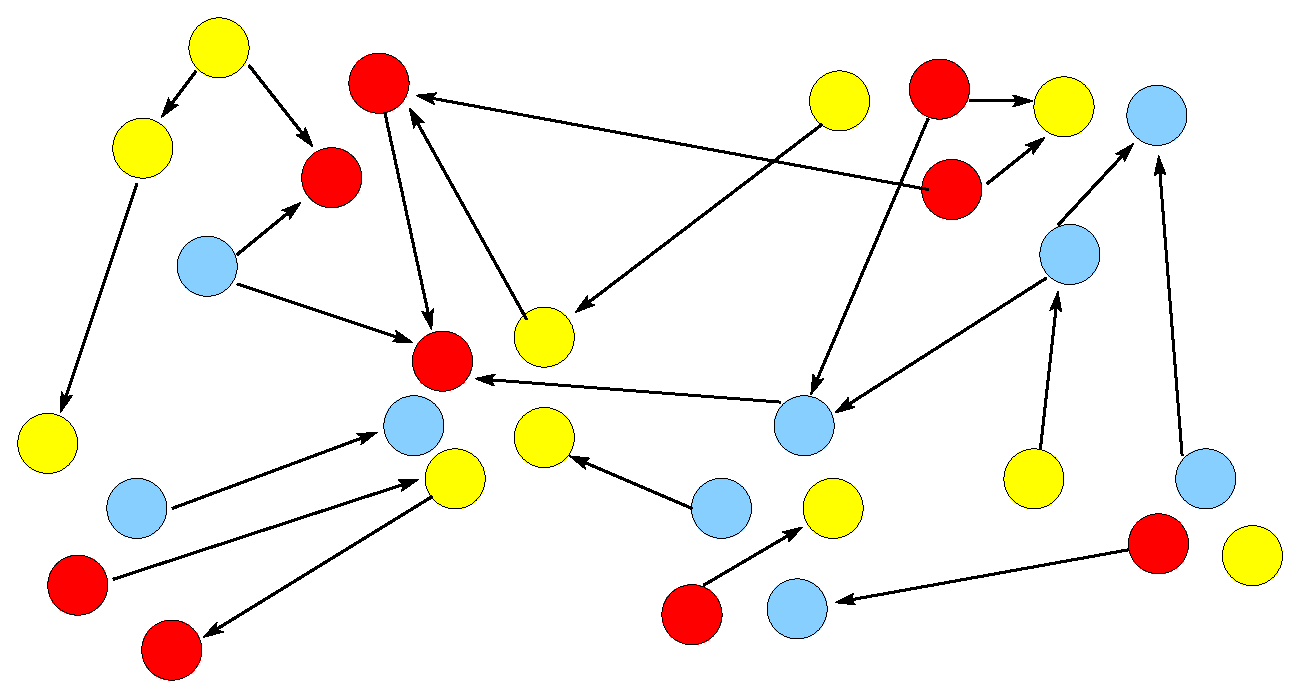
\includegraphics[width=0.45\linewidth]{gm.eps}  }
\caption{ตัวอย่างการใช้ sugfigure}

\end{figure}

\subsection{Equations}
$y=Cx$
\begin{equation}
	F(s) = \int_0^\infty e^{-st} f(t) dt
\end{equation}
the package 'align'
\begin{align}
    x    &= 2 \label{eq:x} \\
    y    &= 3 \label{eq:y} \\
    z    &= x \times y \nonumber \\
        &= p \label{eq:results}
\end{align}
\begin{itemize}
\item To not include an equation number, use \texttt{\nonumber} or \texttt{notag} 
\item Cross referencing can be done using \texttt{ref} or \texttt{eqref} together with \texttt{label}. For example, we refer to~\eqref{eq:x} that $x=2$.
\end{itemize}
the package 'eqnarray' is another environment to arrange equations into array format.
\begin{eqnarray}
\dot{x} &=& Ax + Bu \\
y &=& Cx+Du
\end{eqnarray}
If we want to align all equations into center use the package 'gather'.
\begin{gather}
y = \sum_{n=0}^100 0.5^n + \sin(2\pi n t) + \lim_{n \rightarrow \infty} \frac{\log n}{n} \\
z = \lim_{t \rightarrow \infty} e^{-st} g(t) 
\end{gather}

\subsection{References}
Reference formats are different from reference types. We commonly use the IEEE format, found in 

\url{https://www.ieee.org/documents/ieeecitationref.pdf}

Use BibTex to generate reference list in the document. You will need a list of reference in the format of \texttt{file.bib} containing reference details, which can be exported easily using Google Scholar. When to refer to a paper, use \texttt{cite}. For example, the concept about system identification can be read from~\cite{SoS:89}.

\bibliography{ref}
\bibliographystyle{plain}

% Appendix Section
\section{Appendices}
ภาคผนวกอาจแบ่งได้ออกเป็นหลายส่วน ตามหัวข้อเรื่อง
\subsection{Appendix A}

\subsection{Appendix B}


\end{document}
